\documentclass[aspectratio=169]{beamer}
\usetheme{Madrid}
\usecolortheme{default}
\usepackage[utf8]{inputenc}
\usepackage[T1]{fontenc}
\usepackage[spanish]{babel}
\usepackage{amsmath}
\usepackage{amssymb}
\usepackage{graphicx}
\usepackage{tikz}
\usetikzlibrary{arrows.meta,positioning,calc}

\title{Integración de Control Robótico en Fusion 360}
\subtitle{Fundamentos, modelo matemático e implementación práctica}
\author{RobotArmControl1}
\date{\today}

\begin{document}

\begin{frame}
  \titlepage
\end{frame}

\begin{frame}{Objetivos de aprendizaje}
\begin{itemize}
  \item Comprender la arquitectura completa del sistema de control.
  \item Entender el modelo geométrico y dinámico del brazo robótico.
  \item Relacionar el modelo matemático con el diseño del control PID.
  \item Aplicar criterios prácticos de ajuste, seguridad y validación.
  \item Integrar el control en Fusion 360 con interfaz gráfica y comunicación serial.
\end{itemize}
\end{frame}

\begin{frame}{Ruta de la presentación}
\begin{enumerate}
  \item Planteamiento del problema y arquitectura del sistema.
  \item Modelo matemático: cinemática, Jacobiano y dinámica.
  \item Diseño del controlador PID en tiempo discreto.
  \item Integración en software: UI, Fusion API y serial.
  \item Criterios de seguridad mecánica y validación experimental.
\end{enumerate}
\end{frame}

\begin{frame}{Problema de ingeniería que se resuelve}
\begin{itemize}
  \item El brazo debe alcanzar posiciones objetivo de manera repetible y estable.
  \item El sistema debe aceptar múltiples entradas de mando:
  \begin{enumerate}
    \item movimiento manual por juntas,
    \item objetivo cartesiano $(X,Y)$ por cinemática inversa,
    \item seguimiento por PID en una junta seleccionada.
  \end{enumerate}
  \item Deben respetarse límites físicos para evitar colisiones mecánicas.
  \item El comportamiento esperado del PID es: \textbf{llegar al objetivo y mantenerse en él}.
\end{itemize}
\end{frame}

\begin{frame}{Arquitectura general del proyecto}
\begin{itemize}
  \item \texttt{RobotArmControl1.py}: orquestación de UI, eventos y lazo principal.
  \item \texttt{robot\_arm\_config.py}: límites articulares, parámetros base y configuración.
  \item \texttt{robot\_arm\_kinematics.py}: solución de cinemática inversa del brazo plano 2R.
  \item \texttt{robot\_arm\_pid1.py}: controlador PID, tolerancia y criterio de asentamiento.
  \item \texttt{RobotArmControl1.manifest}: registro del script para ejecución en Fusion.
\end{itemize}
\end{frame}

\begin{frame}{Lazo de control de referencia}
\centering
\begin{tikzpicture}[node distance=1.5cm, >=Latex]
  \node[draw, rounded corners, minimum width=2.6cm, minimum height=0.9cm] (ref) {Referencia $r$};
  \node[draw, rounded corners, minimum width=2.0cm, minimum height=0.9cm, right=1.8cm of ref] (sum) {Error $e$};
  \node[draw, rounded corners, minimum width=2.4cm, minimum height=0.9cm, right=1.8cm of sum] (pid) {Control PID};
  \node[draw, rounded corners, minimum width=3.0cm, minimum height=0.9cm, right=1.8cm of pid] (plant) {Brazo en Fusion};
  \node[draw, rounded corners, minimum width=2.6cm, minimum height=0.9cm, below=1.5cm of plant] (sensor) {Medición $y$};

  \draw[->] (ref) -- (sum);
  \draw[->] (sum) -- node[above] {$u$} (pid);
  \draw[->] (pid) -- (plant);
  \draw[->] (plant) -- (sensor);
  \draw[->] (sensor.west) -| node[pos=0.25,left] {$-$} (sum.south);
\end{tikzpicture}

\vspace{0.5em}
\small{El principio es siempre el mismo: medir, comparar y corregir en cada ciclo.}
\end{frame}

\begin{frame}{Interpretación operativa del PID}
\begin{itemize}
  \item Acción proporcional $K_p$: corrige en función del error instantáneo.
  \item Acción integral $K_i$: corrige errores acumulados en el tiempo.
  \item Acción derivativa $K_d$: anticipa cambios y reduce sobreimpulso.
  \item Combinadas adecuadamente, estas acciones mejoran rapidez y estabilidad.
\end{itemize}
\end{frame}

\begin{frame}{Definición formal de un manipulador 2R}
\begin{itemize}
  \item El término \textbf{2R} significa:
  \begin{enumerate}
    \item \textbf{2}: dos grados de libertad articulares.
    \item \textbf{R}: ambas juntas son revolutas (movimiento angular).
  \end{enumerate}
  \item En el plano, el estado articular se representa como:
\end{itemize}
\[
q = \begin{bmatrix}\theta_1 \\ \theta_2\end{bmatrix}
\]
\begin{itemize}
  \item $\theta_1$: giro de la junta proximal (hombro).
  \item $\theta_2$: giro relativo de la junta distal (codo).
\end{itemize}
\end{frame}

\begin{frame}{Paso 1: sistema de referencia y coordenadas cartesianas}
\begin{itemize}
  \item Se fija un marco base $\{0\}$ con origen en la base del robot.
  \item La punta del brazo (efector final) se describe en coordenadas cartesianas por:
\end{itemize}
\[
p = \begin{bmatrix}x \\ y\end{bmatrix}
\]
\begin{itemize}
  \item $x$: desplazamiento horizontal respecto al origen.
  \item $y$: desplazamiento vertical respecto al origen.
  \item Estas coordenadas indican \textbf{dónde está} la punta en el plano.
\end{itemize}
\end{frame}

\begin{frame}{Paso 2: significado físico de cada variable}
\begin{itemize}
  \item $L_1$: longitud del primer eslabón (hombro a codo).
  \item $L_2$: longitud del segundo eslabón (codo a efector final).
  \item $\theta_1$: orientación absoluta del primer eslabón.
  \item $\theta_2$: flexión relativa entre primer y segundo eslabón.
\end{itemize}
\vspace{0.4em}
\begin{block}{Interpretación directa}
Si se modifican $\theta_1$ y $\theta_2$, cambia la posición $(x,y)$ de la punta. Ese es el vínculo entre espacio articular y espacio cartesiano.
\end{block}
\end{frame}

\begin{frame}{Identificación visual de eslabones en el modelo}
\begin{center}
  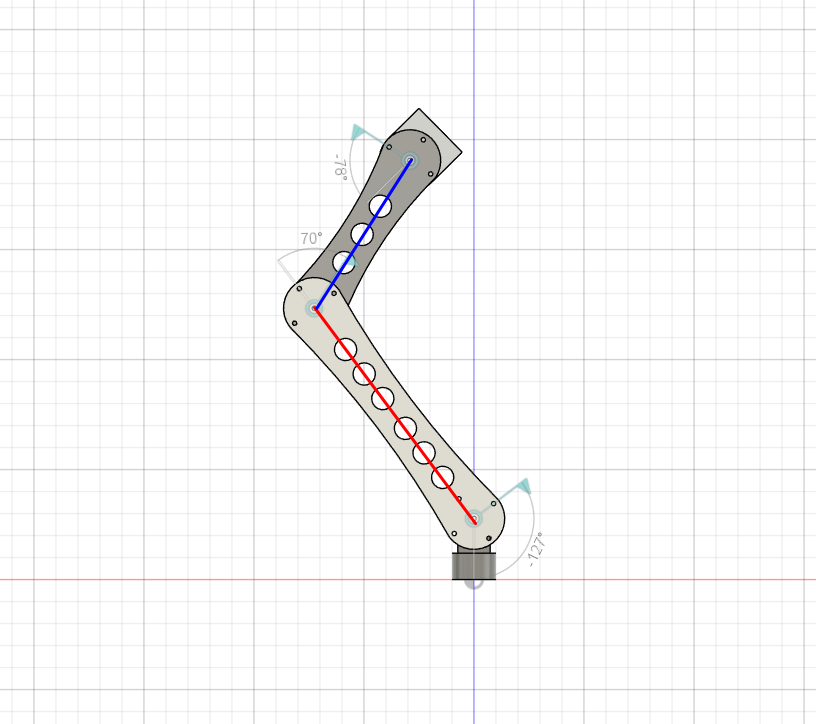
\includegraphics[width=0.50\textwidth]{image.png}
\end{center}
\vspace{0.1em}
\begin{itemize}
  \item Línea roja: representa el eslabón $L_1$.
  \item Línea azul: representa el eslabón $L_2$.
  \item El punto de unión de ambas líneas corresponde al codo.
\end{itemize}
\end{frame}

\begin{frame}{Paso 3: qué representa la referencia cartesiana deseada}
\begin{itemize}
  \item La referencia cartesiana deseada se define como:
\end{itemize}
\[
p_d = \begin{bmatrix}x_d \\ y_d\end{bmatrix}
\]
\begin{itemize}
  \item $x_d, y_d$ son las coordenadas objetivo para la punta del brazo.
  \item Esta referencia no es un ángulo: es una \textbf{posición objetivo en el plano}.
  \item El sistema debe convertir $p_d$ en ángulos objetivo usando cinemática inversa.
\end{itemize}
\end{frame}

\begin{frame}{Paso 4: cadena completa de conversión de referencias}
\centering
\begin{tikzpicture}[node distance=1.35cm, >=Latex]
  \node[draw, rounded corners, minimum width=2.7cm] (pd) {$p_d=[x_d,y_d]^T$};
  \node[draw, rounded corners, right=1.7cm of pd, minimum width=2.6cm] (ik) {Cinemática inversa};
  \node[draw, rounded corners, right=1.7cm of ik, minimum width=2.8cm] (qd) {$q_d=[\theta_{1d},\theta_{2d}]^T$};

  \node[draw, rounded corners, below=1.6cm of pd, minimum width=2.6cm] (q) {$q=[\theta_1,\theta_2]^T$};
  \node[draw, rounded corners, below=1.6cm of ik, minimum width=2.6cm] (pid) {Control PID};
  \node[draw, rounded corners, below=1.6cm of qd, minimum width=2.6cm] (robot) {Brazo 2R};

  \draw[->] (pd) -- (ik);
  \draw[->] (ik) -- (qd);
  \draw[->] (qd.south) -- (robot.north);
  \draw[->] (q) -- (pid);
  \draw[->] (pid) -- (robot);

  \coordinate (fb) at ($(pid.south)+(0,-0.85)$);
  \draw[->] (robot.west) |- (fb) -| (q.south);
\end{tikzpicture}

\vspace{0.5em}
\small{La referencia cartesiana se transforma en referencia articular; el PID ejecuta el seguimiento en lazo cerrado.}
\end{frame}

\begin{frame}{Paso 5: ejemplo numérico mínimo}
\begin{itemize}
  \item Supóngase $L_1=300$ mm y $L_2=200$ mm.
  \item Referencia cartesiana deseada: $p_d=[140,100]^T$ mm.
  \item La cinemática inversa produce un par de ángulos objetivo $(\theta_{1d},\theta_{2d})$.
  \item El PID mueve las juntas hasta que $q \rightarrow q_d$.
  \item Como consecuencia, la punta converge a $p \rightarrow p_d$.
\end{itemize}
\begin{block}{Lectura conceptual}
\textbf{Referencia cartesiana deseada} significa: "quiero la punta aquí".\newline
\textbf{Control articular} significa: "muevo las juntas para lograrlo".
\end{block}
\end{frame}

\begin{frame}{Supuestos numéricos adoptados para la clase}
\begin{itemize}
  \item Geometría del brazo: $L_1=300$ mm, $L_2=200$ mm.
  \item Sistema de referencia: origen en la base, $x$ hacia la derecha, $y$ hacia arriba.
  \item Convención angular: sentido antihorario positivo.
  \item Configuración seleccionada: codo-arriba (elbow-up).
  \item Control PID (según implementación):
  \begin{itemize}
    \item $T_s=0.05$ s,
    \item salida limitada a $\pm 25$ grados por ciclo,
    \item tolerancia de asentamiento $\varepsilon=0.6$ grados,
    \item 3 ciclos consecutivos para declarar convergencia.
  \end{itemize}
\end{itemize}
\end{frame}

\begin{frame}{Cinemática inversa resuelta paso a paso (caso inferido)}
\textbf{Objetivo cartesiano de ejemplo:}
\[
p_d = [250,250]^T\;\text{mm}
\]
\[
r^2=x_d^2+y_d^2=250^2+250^2=125000
\]
\[
\cos\theta_2 = \frac{r^2-L_1^2-L_2^2}{2L_1L_2}
=\frac{125000-90000-40000}{120000}=-0.04167
\]
\[
\theta_2 = -\arccos(-0.04167) = -92.39^\circ
\]
\[
k_1=L_1+L_2\cos\theta_2=300+200(-0.04167)=291.67
\]
\[
k_2=L_2\sin\theta_2=200\sin(-92.39^\circ)\approx-199.83
\]
\[
\theta_1=\operatorname{atan2}(250,250)-\operatorname{atan2}(k_2,k_1)
=45^\circ-(-34.40^\circ)=79.40^\circ
\]
\end{frame}

\begin{frame}{Verificación por cinemática directa del resultado}
\textbf{Resultado IK obtenido:}
\[
\theta_1=79.40^\circ,\quad \theta_2=-92.39^\circ
\]
\[
x=L_1\cos\theta_1+L_2\cos(\theta_1+\theta_2)
\]
\[
x\approx 300\cos79.40^\circ+200\cos(-12.99^\circ)
\approx 55.4+194.8=250.2\;\text{mm}
\]
\[
y=L_1\sin\theta_1+L_2\sin(\theta_1+\theta_2)
\]
\[
y\approx 300\sin79.40^\circ+200\sin(-12.99^\circ)
\approx 294.8-45.0=249.8\;\text{mm}
\]
\begin{itemize}
  \item Error geométrico final del ejemplo: menor a 1 mm por redondeo.
\end{itemize}
\end{frame}

\begin{frame}{Cinemática directa: de ángulos a posición}
\[
\begin{aligned}
x &= L_1\cos\theta_1 + L_2\cos(\theta_1+\theta_2),\\
y &= L_1\sin\theta_1 + L_2\sin(\theta_1+\theta_2).
\end{aligned}
\]
\begin{itemize}
  \item Estas ecuaciones describen la posición de la punta del brazo.
  \item Son el primer bloque matemático para simulación y control.
\end{itemize}
\end{frame}

\begin{frame}{Cinemática inversa: de posición a ángulos}
\[
\cos(\theta_2)=\frac{x^2+y^2-L_1^2-L_2^2}{2L_1L_2}
\]
\[
\theta_2=\pm\arccos(\cos\theta_2)
\]
\[
\theta_1=\operatorname{atan2}(y,x)-\operatorname{atan2}(L_2\sin\theta_2, L_1+L_2\cos\theta_2)
\]
\begin{itemize}
  \item El signo de $\theta_2$ define configuración codo-arriba o codo-abajo.
  \item Esta etapa convierte objetivos $X,Y$ en comandos articulares.
\end{itemize}
\end{frame}

\begin{frame}{Condición de alcanzabilidad}
\[
|L_1-L_2| \leq \sqrt{x^2+y^2} \leq L_1+L_2
\]
\begin{itemize}
  \item Si la referencia está fuera de este intervalo, la IK no tiene solución real.
  \item En la implementación se valida esta condición antes de mover juntas.
\end{itemize}
\end{frame}

\begin{frame}{Jacobiano: relación entre velocidades}
\[
\dot{x} = J(q)\dot{q}
\]
\[
J(q)=
\begin{bmatrix}
- L_1\sin\theta_1 - L_2\sin(\theta_1+\theta_2) & -L_2\sin(\theta_1+\theta_2) \\
\phantom{-}L_1\cos\theta_1 + L_2\cos(\theta_1+\theta_2) & \phantom{-}L_2\cos(\theta_1+\theta_2)
\end{bmatrix}
\]
\begin{itemize}
  \item Permite analizar sensibilidad y propagación de velocidades.
  \item Es clave para identificar zonas de mala condición numérica.
\end{itemize}
\end{frame}

\begin{frame}{Singularidades del manipulador}
\begin{itemize}
  \item Una singularidad es una configuración donde el Jacobiano pierde rango.
  \item En 2R aparecen típicamente en extensión o plegado extremos.
  \item Efecto práctico: control menos robusto y mayor sensibilidad a ruido.
\end{itemize}
\end{frame}

\begin{frame}{Modelo por matrices de transformación homogénea}
\[
{}^{0}T_{2} = {}^{0}T_{1} \cdot {}^{1}T_{2}
\]
\[
{}^{i-1}T_i =
\begin{bmatrix}
\cos\theta_i & -\sin\theta_i & a_i\cos\theta_i \\
\sin\theta_i & \cos\theta_i  & a_i\sin\theta_i \\
0 & 0 & 1
\end{bmatrix}
\]
\begin{itemize}
  \item Este enfoque se extiende de forma natural a robots de mayor complejidad.
\end{itemize}
\end{frame}

\begin{frame}{Modelo dinámico del robot (forma canónica)}
\[
M(q)\ddot{q} + C(q,\dot{q})\dot{q} + g(q) = \tau
\]
\begin{itemize}
  \item $M(q)$: matriz de inercia.
  \item $C(q,\dot{q})\dot{q}$: Coriolis y centrifugos.
  \item $g(q)$: gravedad.
  \item $\tau$: par aplicado por actuadores.
\end{itemize}
\end{frame}

\begin{frame}{Estructura típica de matrices dinámicas (2R)}
\small
\[
M(q)=
\begin{bmatrix}
\alpha + 2\beta\cos\theta_2 & \delta + \beta\cos\theta_2 \\
\delta + \beta\cos\theta_2 & \delta
\end{bmatrix}
\]
\[
C(q,\dot{q})\dot{q}=
\begin{bmatrix}
-\beta\sin\theta_2(2\dot{\theta}_1\dot{\theta}_2 + \dot{\theta}_2^2) \\
\beta\sin\theta_2\dot{\theta}_1^2
\end{bmatrix},\quad
g(q)=
\begin{bmatrix}
g_1(q)\\g_2(q)
\end{bmatrix}
\]
\normalsize
\begin{itemize}
  \item En esta integración se usa principalmente modelo geométrico + PID.
  \item La formulación dinámica queda disponible para extensiones avanzadas.
\end{itemize}
\end{frame}

\begin{frame}{Control PID discreto por junta}
\[
e_k = r_k - y_k
\]
\[
I_k = I_{k-1} + e_k\Delta t,\qquad D_k = \frac{e_k-e_{k-1}}{\Delta t}
\]
\[
u_k = K_p e_k + K_i I_k + K_d D_k
\]
\begin{itemize}
  \item Se aplican saturaciones para preservar límites físicos y robustez.
\end{itemize}
\end{frame}

\begin{frame}{Definición numérica inferida de PID (ejemplo práctico)}
\begin{itemize}
  \item Junta ejemplo: hombro.
  \item Objetivo: $r=60^\circ$ desde condición inicial $y_0=0^\circ$.
  \item Ganancias iniciales inferidas (consistentes con código):
\[
K_p=2.5,\quad K_i=0.2,\quad K_d=0.09
\]
  \item Muestreo y límites:
\[
T_s=0.05\;s,\quad u_{max}=\pm 25\;\text{grados/ciclo}
\]
\end{itemize}
\end{frame}

\begin{frame}{Iteraciones PID calculadas paso a paso}
\textbf{Iteración $k=0$:}
\[
e_0 = 60-0=60
\]
\[
I_0 = 0 + e_0T_s = 60(0.05)=3
\]
\[
D_0 = \frac{e_0-e_{-1}}{T_s}=\frac{60-0}{0.05}=1200
\]
\[
u_0 = K_pe_0 + K_iI_0 + K_dD_0
=2.5(60)+0.2(3)+0.09(1200)=258.6
\]
\[
u_0^{sat}=25\quad(\text{saturación})
\]

\textbf{Iteración $k=1$ (aprox. $y_1\approx 25^\circ$):}
\[
e_1=60-25=35,\quad I_1=3+35(0.05)=4.75
\]
\[
D_1=\frac{35-60}{0.05}=-500
\]
\[
u_1=2.5(35)+0.2(4.75)+0.09(-500)=43.45\Rightarrow u_1^{sat}=25
\]
\begin{itemize}
  \item El término derivativo reduce el sobreimpulso.
  \item La saturación evita comandos peligrosos.
\end{itemize}
\end{frame}

\begin{frame}{Anti-windup y criterio de asentamiento}
\begin{itemize}
  \item Windup: crecimiento excesivo del integrador cuando hay saturación.
  \item Estrategia aplicada: limitar integrador y resetear al converger.
  \item Regla de operación en la implementación:
\end{itemize}
\[
|e|\leq \varepsilon \Rightarrow \text{forzar setpoint y reset PID}
\]
\begin{itemize}
  \item Resultado: reducción de oscilación sostenida alrededor del objetivo.
\end{itemize}
\end{frame}

\begin{frame}{Diagrama de software (integración completa)}
\centering
\begin{tikzpicture}[node distance=1.2cm, >=Latex]
  \node[draw, rounded corners, minimum width=2.5cm] (ui) {UI Tkinter};
  \node[draw, rounded corners, right=2.2cm of ui, minimum width=3.2cm] (logic) {RobotArmControl1.py};
  \node[draw, rounded corners, right=2.2cm of logic, minimum width=3.0cm] (fusion) {API Fusion adsk};
  \node[draw, rounded corners, below=1.4cm of logic, minimum width=2.6cm] (pid) {robot\_arm\_pid1.py};
  \node[draw, rounded corners, below=1.4cm of ui, minimum width=2.8cm] (ik) {robot\_arm\_kinematics.py};
  \node[draw, rounded corners, below=1.4cm of fusion, minimum width=3.0cm] (serial) {Thread Serial + Queue};

  \draw[->] (ui) -- (logic);
  \draw[->] (logic) -- (fusion);
  \draw[->] (pid) -- (logic);
  \draw[->] (ik) -- (logic);
  \draw[->] (serial) -- (logic);
  \draw[->] (logic) -- (pid);
\end{tikzpicture}
\end{frame}

\begin{frame}{Representación en espacio de estado}
\begin{itemize}
  \item Estado: $x=[\theta_1,\theta_2,\dot{\theta}_1,\dot{\theta}_2]^T$.
  \item Entrada: $u=\tau$; salida: $y=[\theta_1,\theta_2]^T$.
  \item En torno a un punto de operación:
\end{itemize}
\[
\dot{x}=Ax+Bu,\qquad y=Cx+Du
\]
\begin{itemize}
  \item Esta forma es base para LQR, observadores y control predictivo.
\end{itemize}
\end{frame}

\begin{frame}{Versión discreta para implementación digital}
\[
x_{k+1}=A_d x_k + B_d u_k, \qquad y_k=C_d x_k + D_d u_k
\]
\begin{itemize}
  \item El tiempo de muestreo $\Delta t$ condiciona estabilidad, ruido y rapidez.
  \item En el sistema actual, el PID se ejecuta de forma periódica con $\Delta t$ fijo.
\end{itemize}
\end{frame}

\begin{frame}{Procedimiento de ajuste de ganancias PID}
\begin{enumerate}
  \item Pon $K_i=0$ y $K_d=0$.
  \item Incrementa $K_p$ hasta obtener rapidez sin oscilación severa.
  \item Sube $K_d$ para amortiguar sobreimpulso.
  \item Ajusta $K_i$ para reducir error estacionario.
  \item Ajusta tolerancia $\varepsilon$ y número de ciclos estables.
\end{enumerate}
\end{frame}

\begin{frame}{Cómo definir valores iniciales de PID en la práctica}
\begin{itemize}
  \item \textbf{Paso A: definir el objetivo de desempeño}
  \begin{itemize}
    \item tiempo de establecimiento deseado,
    \item sobreimpulso máximo permitido,
    \item error estacionario aceptable.
  \end{itemize}
  \item \textbf{Paso B: iniciar con parámetros conservadores}
  \begin{itemize}
    \item fijar $K_i=0$, $K_d=0$ y comenzar con $K_p$ pequeño,
    \item aumentar $K_p$ en incrementos pequeños hasta respuesta adecuada.
  \end{itemize}
  \item \textbf{Paso C: introducir amortiguamiento y precisión}
  \begin{itemize}
    \item incrementar $K_d$ para reducir oscilación y sobreimpulso,
    \item incrementar $K_i$ para corregir error estacionario residual.
  \end{itemize}
  \item \textbf{Paso D: validar con escalones repetidos}
  \begin{itemize}
    \item probar referencias de distinta magnitud,
    \item verificar estabilidad en todo el rango permitido de la junta.
  \end{itemize}
\end{itemize}
\end{frame}

\begin{frame}{Criterios cuantitativos para aceptar un ajuste PID}
\[
e(t)=r(t)-y(t)
\]
\begin{itemize}
  \item Error estacionario: $\lim_{t\to\infty}|e(t)| \leq e_{ss,max}$.
  \item Sobreimpulso relativo:
\[
M_p(\%)=\frac{y_{max}-y_{ss}}{y_{ss}}\times 100
\]
  \item Tiempo de establecimiento $t_s$: tiempo a partir del cual
\[
|e(t)|\leq \varepsilon \quad \text{de forma sostenida}
\]
  \item En este proyecto, la condición práctica se implementa con:
  \begin{itemize}
    \item tolerancia angular $\varepsilon$,
    \item número de ciclos estables consecutivos.
  \end{itemize}
\end{itemize}
\end{frame}

\begin{frame}{Diagnóstico rápido de comportamiento del control}
\begin{itemize}
  \item Oscilación persistente: disminuir $K_p$ y/o aumentar $K_d$.
  \item Respuesta lenta: aumentar $K_p$ con incrementos pequeños.
  \item Error estacionario: aumentar $K_i$ de forma gradual.
  \item Sensibilidad a ruido: reducir $K_d$ o filtrar derivada.
\end{itemize}
\end{frame}

\begin{frame}{Integración serial: cadena de procesamiento}
\begin{enumerate}
  \item El emisor transmite tramas \texttt{BASE,HOMBRO,CODO}.
  \item Hilo serial parsea y valida formato.
  \item Los datos válidos se publican en cola thread-safe.
  \item El hilo principal consume cola y actualiza estado y juntas.
\end{enumerate}
\end{frame}

\begin{frame}{Calibración respecto a línea de referencia}
\begin{itemize}
  \item Se mide diferencia entre cero visual y cero matemático.
  \item Se define offset en la UI.
  \item Conversión implementada:
\end{itemize}
\[
\theta_{ref}=\theta_{joint}+offset
\]
\begin{itemize}
  \item Garantiza coherencia entre visualización y variable controlada.
\end{itemize}
\end{frame}

\begin{frame}{Secuencia recomendada de puesta en marcha}
\begin{enumerate}
  \item Verificar nombres de juntas y límites mecánicos.
  \item Probar modo manual para validación básica.
  \item Probar modo cartesiano para validar IK.
  \item Activa PID de una junta y ajusta.
  \item Repetir ajuste en cada junta crítica.
  \item Integrar comunicación serial al final de la etapa de ajuste.
\end{enumerate}
\end{frame}

\begin{frame}{Checklist de validación de integración}
\begin{itemize}
  \item Script detectado y ejecutable en la pestaña Scripts de Fusion.
  \item Interfaz estable y respuesta continua de controles.
  \item Validación de IK con manejo correcto de puntos inalcanzables.
  \item PID converge y mantiene referencia sin oscilación permanente.
  \item Serial conecta y desconecta de forma robusta.
  \item Límites de seguridad evitan movimientos en zonas de colisión.
\end{itemize}
\end{frame}

\begin{frame}{Conclusiones}
\begin{itemize}
  \item Se integró un sistema de control robótico funcional en Fusion 360.
  \item El diseño combina modelo matemático, control y arquitectura de software.
  \item La solución es modular y apta para evolución hacia control avanzado.
\end{itemize}
\vspace{0.5em}
\centering
\Large{Proyección: LQR/MPC, estimación de estado y registro automático de desempeño}
\end{frame}

\begin{frame}
\centering
\Huge Preguntas
\end{frame}

\end{document}
